\documentclass[11pt, oneside, numbers=noenddot]{scrbook}  

\usepackage{style}

\def\Title{Static Routes}	
\def\Subtitle{Netzwerktechnik}


\begin{document}


\titlehead{%
\begin{minipage}[c]{0.20\linewidth}

\includegraphics[width=0.8\linewidth]{htl_c_cmyk_rein.pdf}
\end{minipage}
\begin{minipage}[c]{0.5\linewidth}
\begin{center}
{\bfseries\sffamily\large Höhere  technische  Bundeslehranstalt\\
und  Bundesfachschule\\
{\normalsize im Hermann Fuchs Bundesschulzentrum} }
\end{center}
\end{minipage}
\begin{minipage}[c]{0.2\linewidth}
\hfill 
\includegraphics[width=0.8\linewidth]{htl-bildung-mit-zukunft.png}
\end{minipage}\\
}
\title{\vspace{4em}\Title}

\subtitle{\Subtitle}


\author{\\[2,5em] 
\emph{Erstellt von:} \\[0,5em]
Michel Rögl-Brunner, BEd
}
\date{\vspace{3\baselineskip}\small Letzte Änderung: \todayshort}

\begin{titlepage}	
\maketitle
\end{titlepage}
\IfFileExists{revisions.tex}{\clearpage\input{revisions.tex}}{}
\cleardoublepage
\pdfbookmark[1]{Inhaltsverzeichnis}{toc}
\tableofcontents
\clearpage
\pagenumbering{arabic}

\chapter{Grundlagen}
\section{Was ist Static Routing?}
Statisches Routing bedeutet, dass Routen manüll am Router eingetragen werden. Der Router lernt diese Wege nicht dynamisch, sondern verwendet exakt die konfigurierten Einträge.

Auf Cisco-Routern wird eine statische Route typischerweise so gesetzt:
\begin{verbatim}
ip route <zielnetz> <netzmaske> <next-hop-ip oder ausgangsinterface>
\end{verbatim}

Beispiel:
\begin{verbatim}
ip route 10.30.10.0 255.255.255.0 172.16.0.13
\end{verbatim}
Der Router weiss dann, dass das Netz \texttt{10.30.10.0/24} über den nächsten Router mit der Adresse \texttt{172.16.0.13} erreichbar ist.

\section{Static vs. Dynamic Routing}
\begin{itemize}
\item \textbf{Static Routing:} wenig Overhead, sehr kontrollierbar, aber mehr manüller Aufwand.
\item \textbf{Dynamic Routing:} Routen werden automatisch gelernt (z.\,B.\ OSPF, EIGRP, RIP), dafür mehr Protokollverkehr und komplexere Konfiguration.
\end{itemize}

Für kleine bis mittlere Topologien ist Static Routing gut geeignet, wenn der Netzaufbau stabil ist und sich selten ändert.

\section{Default Route und spezifische Routen}
Eine spezifische Route gilt für ein bestimmtes Zielnetz. Eine Default Route (\texttt{0.0.0.0/0}) ist eine Auffangroute für alle Ziele, für die keine spezifischere Route vorhanden ist.

In dieser Übung werden \textbf{spezifische statische Routen} zu allen anderen Gruppennetzen konfiguriert.

\section{Subinterfaces am Router}
Bevor statische Routen zwischen den Gruppen funktionieren, muss in jeder Gruppe zuerst das lokale Inter-VLAN-Routing laufen. Dafuer wird Router-on-a-Stick mit Subinterfaces verwendet.

Ein Subinterface ist ein virtuelles Teilinterface auf einem physischen Port (z.\,B.\ \texttt{Gi0/0.10} oder \texttt{Fa0/0.10}). Es hat zwei Aufgaben:
\begin{itemize}
\item VLAN-Zuordnung ueber \texttt{encapsulation dot1Q <VLAN-ID>}
\item Gateway-IP fuer genau dieses VLAN
\end{itemize}

Beispiel:
\begin{verbatim}
interface gi0/0.10 (oder fa0/0.10)
 encapsulation dot1Q 10
 ip address 10.10.10.254 255.255.255.0

interface gi0/0.20 (oder fa0/0.20)
 encapsulation dot1Q 20
 ip address 10.10.20.254 255.255.255.0
\end{verbatim}
Erst wenn diese lokalen Gateways funktionieren, koennen Pakete anschliessend per statischer Route in die anderen Gruppen weitergeleitet werden.

\chapter{Topologie und Adressierung}
\section{Rahmenbedingungen}
Es gibt 4 Gruppen. Jede Gruppe erhält:
\begin{itemize}
\item 1x Cisco Catalyst 3550 Switch
\item 1x Cisco 2800 Series Router
\item 2 lokale Netze (VLANs) im Router-on-a-Stick-Design
\item pro lokalem Netz 1 PC
\end{itemize}

Adressregel in jedem lokalen Netz:
\begin{itemize}
\item PC: \texttt{.1}
\item Switch (SVI): \texttt{.253}
\item Router-Subinterface (Gateway): \texttt{.254}
\end{itemize}

Transportnetz zwischen den Gruppenroutern:
\begin{itemize}
\item \texttt{172.16.0.0/24}
\end{itemize}

\section{Subnetzplan}
\begin{itemize}
\item Gruppe 1: \texttt{10.10.10.0/24} und \texttt{10.10.20.0/24}
\item Gruppe 2: \texttt{10.20.10.0/24} und \texttt{10.20.20.0/24}
\item Gruppe 3: \texttt{10.30.10.0/24} und \texttt{10.30.20.0/24}
\item Gruppe 4: \texttt{10.40.10.0/24} und \texttt{10.40.20.0/24}
\end{itemize}

\section{Interface-Belegung}
\subsection{Gruppe 1}
\begin{longtable}{|l|l|l|}
\hline
Verbindung & Linke Seite & Rechte Seite \\
\hline
G1-PC1 zu G1-SW & G1-PC1 NIC & G1-SW Fa0/1 \\
\hline
G1-PC2 zu G1-SW & G1-PC2 NIC & G1-SW Fa0/2 \\
\hline
G1-SW zu G1-RTR (Trunk) & G1-SW Fa0/24 & G1-RTR Gi0/0 (oder Fa0/0) \\
\hline
G1-RTR ins Transportnetz & G1-RTR Gi0/1 (oder Fa0/1) & Transport-Segment 172.16.0.0/24 \\
\hline
\end{longtable}

\subsection{Gruppe 2}
\begin{longtable}{|l|l|l|}
\hline
Verbindung & Linke Seite & Rechte Seite \\
\hline
G2-PC1 zu G2-SW & G2-PC1 NIC & G2-SW Fa0/1 \\
\hline
G2-PC2 zu G2-SW & G2-PC2 NIC & G2-SW Fa0/2 \\
\hline
G2-SW zu G2-RTR (Trunk) & G2-SW Fa0/24 & G2-RTR Gi0/0 (oder Fa0/0) \\
\hline
G2-RTR ins Transportnetz & G2-RTR Gi0/1 (oder Fa0/1) & Transport-Segment 172.16.0.0/24 \\
\hline
\end{longtable}

\subsection{Gruppe 3}
\begin{longtable}{|l|l|l|}
\hline
Verbindung & Linke Seite & Rechte Seite \\
\hline
G3-PC1 zu G3-SW & G3-PC1 NIC & G3-SW Fa0/1 \\
\hline
G3-PC2 zu G3-SW & G3-PC2 NIC & G3-SW Fa0/2 \\
\hline
G3-SW zu G3-RTR (Trunk) & G3-SW Fa0/24 & G3-RTR Gi0/0 (oder Fa0/0) \\
\hline
G3-RTR ins Transportnetz & G3-RTR Gi0/1 (oder Fa0/1) & Transport-Segment 172.16.0.0/24 \\
\hline
\end{longtable}

\subsection{Gruppe 4}
\begin{longtable}{|l|l|l|}
\hline
Verbindung & Linke Seite & Rechte Seite \\
\hline
G4-PC1 zu G4-SW & G4-PC1 NIC & G4-SW Fa0/1 \\
\hline
G4-PC2 zu G4-SW & G4-PC2 NIC & G4-SW Fa0/2 \\
\hline
G4-SW zu G4-RTR (Trunk) & G4-SW Fa0/24 & G4-RTR Gi0/0 (oder Fa0/0) \\
\hline
G4-RTR ins Transportnetz & G4-RTR Gi0/1 (oder Fa0/1) & Transport-Segment 172.16.0.0/24 \\
\hline
\end{longtable}

\section{Logische Netzzeichnung}
\begin{figure}[H]
\centering
\IfFileExists{Work/Aufgaben/NWT/Static-Routes/Static-routing.png}{%
  
\includegraphics[width=\textwidth]{Work/Aufgaben/NWT/Static-Routes/Static-routing.png}%
}{%
  \IfFileExists{Static-routing.png}{%
    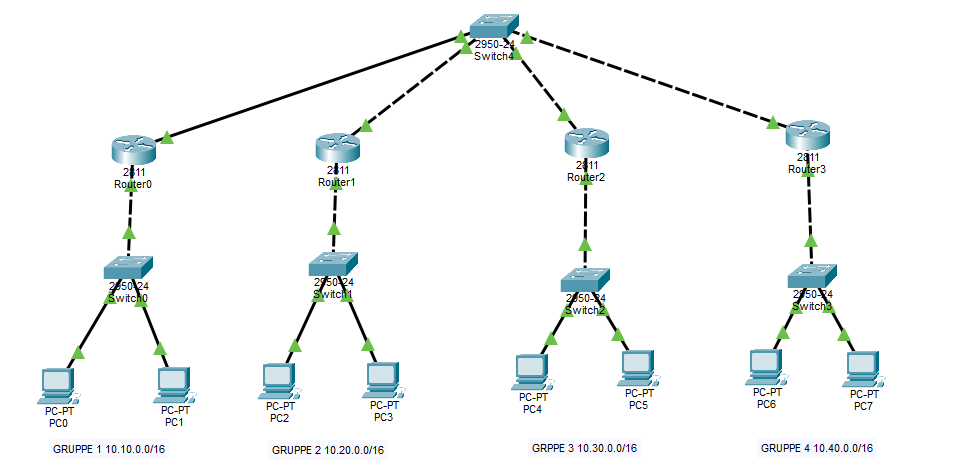
\includegraphics[width=\textwidth]{Static-routing.png}%
  }{%
    \fbox{\parbox{0.9\textwidth}{%
      Bilddatei fehlt: \texttt{Static-routing.png}.\\
      Erwarteter Pfad: \texttt{Work/Aufgaben/NWT/Static-Routes/Static-routing.png}
    }}%
  }%
}
\caption{Topologie fuer die Static-Routing-Uebung}
\end{figure}

\chapter{IP-Tabellen pro Gruppe}
\section{Gruppe 1}
\begin{longtable}{|l|l|l|l|l|}
\hline
Gerät & Interface & IP-Adresse & Maske & Default Gateway \\
\hline
G1-PC1 & NIC & 10.10.10.1 & 255.255.255.0 & 10.10.10.254 \\
\hline
G1-PC2 & NIC & 10.10.20.1 & 255.255.255.0 & 10.10.20.254 \\
\hline
G1-SW & VLAN 10 (SVI) & 10.10.10.253 & 255.255.255.0 & 10.10.10.254 \\
\hline
G1-SW & VLAN 20 (SVI) & 10.10.20.253 & 255.255.255.0 & 10.10.20.254 \\
\hline
G1-RTR & Gi0/0.10 (oder Fa0/0.10) & 10.10.10.254 & 255.255.255.0 & - \\
\hline
G1-RTR & Gi0/0.20 (oder Fa0/0.20) & 10.10.20.254 & 255.255.255.0 & - \\
\hline
G1-RTR & Gi0/1 (oder Fa0/1) & 172.16.0.11 & 255.255.255.0 & - \\
\hline
\end{longtable}

\section{Gruppe 2}
\begin{longtable}{|l|l|l|l|l|}
\hline
Gerät & Interface & IP-Adresse & Maske & Default Gateway \\
\hline
G2-PC1 & NIC & 10.20.10.1 & 255.255.255.0 & 10.20.10.254 \\
\hline
G2-PC2 & NIC & 10.20.20.1 & 255.255.255.0 & 10.20.20.254 \\
\hline
G2-SW & VLAN 10 (SVI) & 10.20.10.253 & 255.255.255.0 & 10.20.10.254 \\
\hline
G2-SW & VLAN 20 (SVI) & 10.20.20.253 & 255.255.255.0 & 10.20.20.254 \\
\hline
G2-RTR & Gi0/0.10 (oder Fa0/0.10) & 10.20.10.254 & 255.255.255.0 & - \\
\hline
G2-RTR & Gi0/0.20 (oder Fa0/0.20) & 10.20.20.254 & 255.255.255.0 & - \\
\hline
G2-RTR & Gi0/1 (oder Fa0/1) & 172.16.0.12 & 255.255.255.0 & - \\
\hline
\end{longtable}
\newpage
\section{Gruppe 3}
\begin{longtable}{|l|l|l|l|l|}
\hline
Gerät & Interface & IP-Adresse & Maske & Default Gateway \\
\hline
G3-PC1 & NIC & 10.30.10.1 & 255.255.255.0 & 10.30.10.254 \\
\hline
G3-PC2 & NIC & 10.30.20.1 & 255.255.255.0 & 10.30.20.254 \\
\hline
G3-SW & VLAN 10 (SVI) & 10.30.10.253 & 255.255.255.0 & 10.30.10.254 \\
\hline
G3-SW & VLAN 20 (SVI) & 10.30.20.253 & 255.255.255.0 & 10.30.20.254 \\
\hline
G3-RTR & Gi0/0.10 (oder Fa0/0.10) & 10.30.10.254 & 255.255.255.0 & - \\
\hline
G3-RTR & Gi0/0.20 (oder Fa0/0.20) & 10.30.20.254 & 255.255.255.0 & - \\
\hline
G3-RTR & Gi0/1 (oder Fa0/1) & 172.16.0.13 & 255.255.255.0 & - \\
\hline
\end{longtable}

\section{Gruppe 4}
\begin{longtable}{|l|l|l|l|l|}
\hline
Gerät & Interface & IP-Adresse & Maske & Default Gateway \\
\hline
G4-PC1 & NIC & 10.40.10.1 & 255.255.255.0 & 10.40.10.254 \\
\hline
G4-PC2 & NIC & 10.40.20.1 & 255.255.255.0 & 10.40.20.254 \\
\hline
G4-SW & VLAN 10 (SVI) & 10.40.10.253 & 255.255.255.0 & 10.40.10.254 \\
\hline
G4-SW & VLAN 20 (SVI) & 10.40.20.253 & 255.255.255.0 & 10.40.20.254 \\
\hline
G4-RTR & Gi0/0.10 (oder Fa0/0.10) & 10.40.10.254 & 255.255.255.0 & - \\
\hline
G4-RTR & Gi0/0.20 (oder Fa0/0.20) & 10.40.20.254 & 255.255.255.0 & - \\
\hline
G4-RTR & Gi0/1 (oder Fa0/1) & 172.16.0.14 & 255.255.255.0 & - \\
\hline
\end{longtable}

\chapter{Aufgabe: Router-on-a-Stick und Static Routing}
\section{Teil A: Router-on-a-Stick in der eigenen Gruppe}
\begin{enumerate}
\item Legt auf dem Switch zwei VLANs an (z.\,B.\ VLAN 10 und VLAN 20).
\item Konfiguriert den Port zum Router als Trunk.
\item Erstellt am Router zwei Subinterfaces (z.\,B.\ \texttt{Gi0/0.10} oder \texttt{Fa0/0.10}) mit 802.1Q und Gateway-IP \texttt{.254}.
\item Vergibt die IP-Adressen an beide PCs gemäss Tabelle.
\item Prüft innerhalb der Gruppe:
  \begin{itemize}
  \item PC1 pingt eigenes Gateway
  \item PC2 pingt eigenes Gateway
  \item PC1 pingt PC2 (Inter-VLAN Routing über Router)
  \end{itemize}
\end{enumerate}

\section{Teil B: Transportnetz und statische Routen}
\begin{enumerate}
\item Konfiguriert das Interface ins Transportnetz \texttt{172.16.0.0/24} am Gruppenrouter.
\item Tragt auf jedem Router statische Routen zu allen \textbf{fremden} Netzen ein.
\item Verwendet als Next Hop die Transport-IP des jeweils zuständigen Zielrouters.
\end{enumerate}

\section{Teil C: Funktionsprüfung}
\begin{enumerate}
\item Erstellt eine Ping-Matrix: Jeder PC soll alle anderen PCs erreichen.
\item Dokumentiert fehlgeschlagene Pings und behebt die Fehler.
\item Endabnahme: Vollständige Erreichbarkeit aller 8 PCs.
\end{enumerate}

\section{Hilfreiche Cisco-Kommandos}
\begin{verbatim}
show ip route
show running-config
show vlan brief
show interfaces trunk
ping <ziel-ip>
\end{verbatim}


\end{document}